
\documentclass[conference]{IEEEtran}
\IEEEoverridecommandlockouts
\usepackage{cite}
\usepackage{multicol}
\usepackage{etoolbox}
\usepackage{relsize}
\usepackage{empheq}
\newcommand*\widefbox[1]{\fbox{\hspace{1em}#1\hspace{1em}}}
\usepackage{amsmath,amssymb,amsfonts}
\usepackage[ruled,vlined]{algorithm2e}
\usepackage{algorithmic}
\usepackage{graphicx}
%\usepackage[warn]{textcomp}
\usepackage{textcomp}
\usepackage{xcolor}
\usepackage{gensymb}
\usepackage{siunitx}
\def\BibTeX{{\rm B\kern-.05em{\sc i\kern-.025em b}\kern-.08em
    T\kern-.1667em\lower.7ex\hbox{E}\kern-.125emX}}
    
\usepackage[utf8]{inputenc}
\usepackage{amsmath}
%\usepackage{mathtools}
\usepackage{braket}
\usepackage{graphicx}
\usepackage{amsfonts}
\usepackage[section]{placeins} 
\usepackage{pgfplots}
\usepackage{csquotes}
\usepackage{hhline}
\usepackage{amssymb}
\usepackage{listings}
\usepackage{color}
\definecolor{codegreen}{rgb}{0,0.6,0}
\definecolor{codegray}{rgb}{0.5,0.5,0.5}
\definecolor{codepurple}{rgb}{0.58,0,0.82}
\definecolor{backcolour}{rgb}{0.95,0.95,0.92}
\usepackage{tabularx}
\usepackage[noadjust]{cite}

\lstdefinestyle{mystyle}{
    backgroundcolor=\color{backcolour},   
    commentstyle=\color{codegreen},
    keywordstyle=\color{magenta},
    numberstyle=\tiny\color{codegray},
    stringstyle=\color{codepurple},
    basicstyle=\footnotesize,
    breakatwhitespace=false,         
    breaklines=true,                 
    captionpos=b,                    
    keepspaces=true,                 
    numbers=left,                    
    numbersep=5pt,                  
    showspaces=false,                
    showstringspaces=false,
    showtabs=false,                  
    tabsize=2
}

\lstset{style=mystyle}
%\usepackage{subfigure}
\usepackage{subcaption}
\newtheorem{teorema}{Theorem}
%%\newcommand*{\Comb}[2]{{}^{#1}C_{#2}}
\usepackage{dcolumn}
\usepackage[qm]{qcircuit}
\usepackage{tabularx}
\setcounter{secnumdepth}{3}
\usepackage[colorlinks=true,linkcolor=blue,citecolor=blue,urlcolor=blue]{hyperref}
\usepackage{longtable}
\usepackage{braket}
%\newtheorem{teorema}{Theorem}
\usepackage{float}
\newcolumntype{C}{>{\centering\arraybackslash}X}
\pgfplotsset{compat=1.15}
\usepackage{multirow}
\pagestyle{plain}
\usepackage{authblk}
\title{Quantum-Enhanced Semantic Segmentation: Harnessing the Power of Quantum-Classical Hybrid U-Net for Medical Imaging}
%\author[1]{Subhash Shankar Pandey}
%\author[1]{Dhrubajyoti Sadhukhan}
%\author[1]{Prasanta K. Panigrahi}
%\affil[1]{Department of Physical Sciences, Indian Institute of Science Education and Research Kolkata, India}
%\affil[*]{pprasanta@iiserkol.ac.in}


\begin{document}
\maketitle
\begin{abstract}
Quantum computing holds great promise for revolutionizing various domains, including medical imaging. In this paper, we propose a novel quantum-classical hybrid U-Net architecture that leverages quantum computing techniques to enhance the performance of semantic segmentation tasks. Specifically, we introduce a quantum layer to replace the bottleneck layer in the traditional U-Net architecture. By utilizing the inherent parallelism and optimization capabilities of quantum computing, our hybrid model aims to address the limitations of U-Net, such as computational complexity and the handling of imbalanced datasets. The quantum layer enables more efficient parameter optimization, reducing the computational burden and improving segmentation accuracy. Furthermore, quantum computing's ability to capture intricate patterns and correlations offers the potential for better handling of fine-grained details and densely packed objects in medical images. Through experiments on medical imaging datasets, we demonstrate the effectiveness and advantages of the proposed quantum-classical hybrid U-Net architecture, showcasing its potential to advance semantic segmentation in medical imaging and pave the way for improved diagnostic and treatment planning tools.
\end{abstract}

Keywords: Quantum AES, Encryption, Cryptography, Machine learning algorithm.
%\end{abstract}
%\maketitle
\section{Introduction}

Semantic segmentation, the task of assigning a label to each pixel in an image, has been a fundamental problem in computer vision for decades. With the advent of deep learning techniques, particularly convolutional neural networks (CNNs), significant progress has been made in addressing this challenge. However, medical image segmentation poses unique difficulties due to the presence of complex anatomical structures, variations in image quality, and scarcity of annotated data.
In 2015, Olaf Ronneberger et al. introduced the U-Net architecture, a groundbreaking CNN design tailored specifically for biomedical image segmentation. Inspired by the encoder-decoder framework, U-Net employs a symmetrical structure that combines local information with global context, enabling accurate delineation of object boundaries while capturing fine details within the segmented regions. This architecture has since gained widespread recognition and has become a benchmark for semantic segmentation tasks, particularly in medical imaging. 
While U-Net has proven to be a highly effective architecture for semantic segmentation in medical imaging, it does have certain limitations. One major drawback is its reliance on a large number of parameters, which can make training and inference computationally expensive and memory-intensive. % quantify this %
Additionally, U-Net may struggle when dealing with highly imbalanced datasets or scenarios where the objects of interest are small and densely packed, as it primarily focuses on capturing global context.
To address these challenges, We proposed a quantum-classical hybrid U-Net architecture. These architectures combine the strengths of classical deep learning models like U-Net with quantum computing techniques to enhance performance. By leveraging quantum computing's inherent parallelism and optimization capabilities, these hybrid models can potentially improve the efficiency and effectiveness of U-Net.
Quantum-classical hybrid U-Net architectures offer several advantages over the traditional U-Net. Quantum algorithms, such as quantum machine learning algorithms or quantum-inspired optimization, can be applied to improve parameter optimization, reducing the computational burden. Additionally, quantum computing's ability to handle complex probability distributions can help address imbalanced datasets by providing more accurate representations of rare classes. Furthermore, quantum-classical hybrid U-Net architectures can enable better handling of fine-grained details and densely packed objects, as quantum computing techniques excel at capturing intricate patterns and correlations.
By incorporating quantum computing techniques into the U-Net architecture, the limitations of the traditional U-Net can be mitigated. The combination of classical and quantum approaches in a hybrid framework presents exciting opportunities for advancing semantic segmentation in medical imaging, offering more efficient and accurate solutions for critical clinical applications. 


\subsection{Overview on classical AES}
The U-Net architecture derives its name from its distinctive "U" shape, characterized by a contracting path and an expansive path. The contracting path, also known as the encoder, consists of successive convolutional and pooling layers that extract hierarchical features and progressively reduce the spatial dimensions. This encoding process allows the network to capture high-level context while maintaining spatial information.
The expansive path, or the decoder, is responsible for recovering spatial details and generating segmentation masks. It employs transposed convolutions (also known as deconvolutions) to upsample the feature maps, combined with skip connections that concatenate feature maps from the contracting path to preserve fine-grained information. This allows the network to leverage both low-level and high-level features for precise segmentation.

\begin{figure}[]

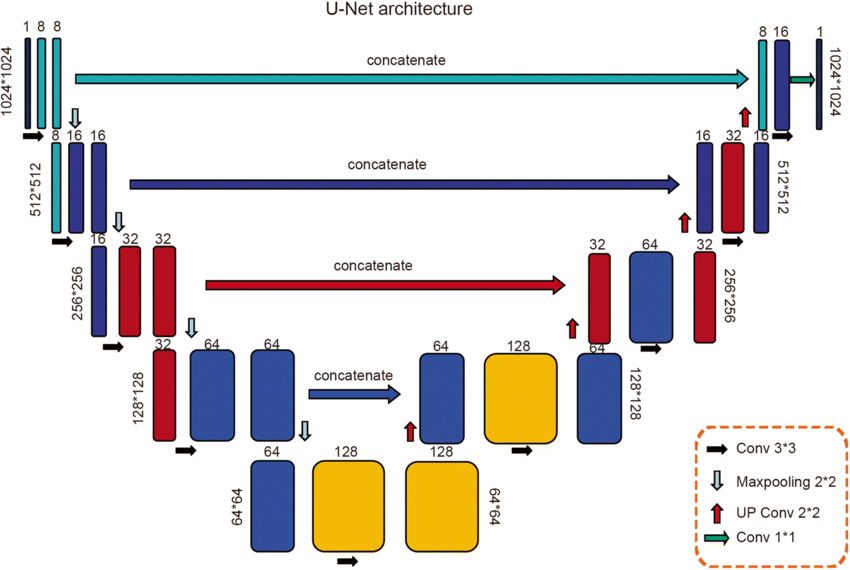
\includegraphics[scale = .3]{U-Net-architecture-consisting-of-two-parts-with-encoding-left-hand-side-and-decoding.png}
\caption{U-Net-architecture-consisting-of-two-parts-with-encoding-left-hand-side-and-decoding}
\label{fig .1}
\end{figure}


The U-Net architecture is further enhanced by the incorporation of skip connections, which help overcome the limitations of traditional encoders and decoders. These skip connections establish direct connections between the contracting and expansive paths at various levels, enabling the decoder to access multi-scale information during upsampling. Consequently, the network is capable of capturing both global context and local details, resulting in highly accurate and context-aware segmentations.
\subsection{Applications in Medical Imaging}
U-Net is a convolutional neural network (CNN) architecture that has proven to be highly effective in various medical imaging applications. Its unique design enables precise segmentation of medical images, making it particularly useful in tasks such as image segmentation, object detection, and image-to-image translation. Here are some applications of U-Net in medical imaging:
Image Segmentation: U-Net is commonly used for pixel-level segmentation tasks, where the goal is to assign a label to each pixel in an image. This is valuable in medical imaging for segmenting organs, tumors, lesions, and other structures of interest. By training the U-Net on annotated images, it can accurately identify and outline specific regions within the medical images.
\subsubsection{Tumor Detection and Classification:}
 U-Net can be employed to detect and classify tumors in medical images such as MRI, CT scans, or ultrasound. By training the network on labeled images, it learns to identify tumor boundaries and distinguish between different tumor types. This assists radiologists in early diagnosis, treatment planning, and monitoring of tumor progression.
 \subsubsection{Lesion Segmentation:}
 In dermatology, U-Net can aid in the segmentation and identification of skin lesions. By training on images with annotated lesion boundaries, the network can accurately delineate the extent and shape of the lesions. This information is crucial for diagnosing skin conditions and tracking the progression of diseases like melanoma.
  \subsubsection{Vessel Segmentation:}
 U-Net can be used to segment blood vessels from medical images such as angiograms or retinal images. This is essential in diagnosing and monitoring vascular diseases, such as diabetic retinopathy or arterial occlusions. Accurate vessel segmentation assists in quantifying vessel properties and identifying abnormalities.
 \subsubsection{Organ Segmentation:}
 U-Net is highly effective in segmenting organs from medical images such as CT or MRI scans. It can identify and outline structures like the liver, kidneys, heart, or lungs, enabling automated measurements, surgical planning, and quantitative analysis. Precise organ segmentation is crucial for medical interventions and treatment evaluation.
 \subsubsection{Image Reconstruction and Enhancement:}
 U-Net can be employed to improve the quality of medical images by reconstructing high-resolution images from low-resolution inputs or denoising noisy images. By training the network on paired images, it learns to capture the details and enhance the visual quality, aiding in accurate diagnosis and interpretation.
 \subsubsection{Image Registration:}
 U-Net can be used for aligning and registering medical images from different modalities or time points. By training the network on paired images, it learns to establish correspondences between images, enabling precise spatial alignment. Image registration is valuable for tracking disease progression and comparing images for treatment planning.
These are just a few examples of how U-Net is applied in medical imaging. Its versatility, accuracy, and ability to handle limited training data make it a popular choice for various segmentation and image analysis tasks in the medical field.
\section{Prerequisite}
\subsection{Quantum Layer}
A quantum layer in a hybrid neural network is a layer that utilizes quantum operations and quantum states to process and manipulate data. It works by applying quantum gates, which are fundamental units of quantum circuits, to quantum bits or qubits. Qubits can exist in superposition states and be entangled, allowing for simultaneous representation of multiple values and correlations between qubits.\\

The advantages of a quantum layer in a hybrid neural network include the potential for enhanced computational capabilities compared to classical layers alone. Quantum layers can tackle problems that are difficult for classical neural networks, particularly in optimization and simulation of quantum systems. Quantum algorithms like the quantum approximate optimization algorithm (QAOA) and quantum support vector machines (QSVM) can be utilized more efficiently.\\

One of the key benefits of a quantum layer is its ability to introduce nonlinearity in the computations. Nonlinearity is crucial for neural networks to model complex relationships in data. Quantum gates, such as the Hadamard gate and controlled-NOT gate, introduce nonlinearity by transforming the qubit states in a way that is nonlinear with respect to the input. This nonlinearity allows quantum layers to capture more intricate patterns and make the network more expressive.\\

By incorporating a quantum layer into a hybrid neural network, the network can take advantage of both classical and quantum computing capabilities. Classical layers handle pre-processing, feature extraction, and post-processing, while quantum layers perform quantum computations. This combination harnesses the strengths of both approaches, potentially leading to improved performance and efficiency in solving specific tasks.\\

\subsection{U-Net Lite}
U-Net Lite is a lightweight version of the U-Net architecture, which is widely used for semantic segmentation tasks in computer vision. While the original U-Net architecture has a more extensive channel extension, U-Net Lite reduces the number of channels, typically starting from 4 and going up to 128, to reduce the model's complexity and memory requirements.\\

Semantic segmentation involves assigning a class label to each pixel in an image, enabling detailed understanding and analysis of the image's content. U-Net Lite follows the same encoder-decoder structure as the original U-Net but with a simplified channel configuration.\\

In U-Net Lite, the encoder component consists of several convolutional layers, each followed by a rectified linear unit (ReLU) activation function and a max-pooling operation. These layers extract features from the input image while progressively reducing the spatial dimensions.\\

The decoder component in U-Net Lite consists of upsampled feature maps, achieved through either transposed convolutions or upsampling followed by regular convolutions. These operations gradually restore the spatial resolution back to the original size of the input image.\\

Although U-Net Lite has a reduced number of channels compared to the original U-Net, it still maintains skip connections, which are crucial for preserving and combining features at different scales. Skip connections help U-Net Lite capture both high-level contextual information and low-level details, enhancing the accuracy of the segmentation results.\\

U-Net Lite is commonly used in scenarios where computational resources are limited, such as on edge devices or in situations with restricted memory capacity. By reducing the number of channels, the model becomes more lightweight and efficient, allowing for faster inference and lower memory footprint.\\

\begin{figure}[]

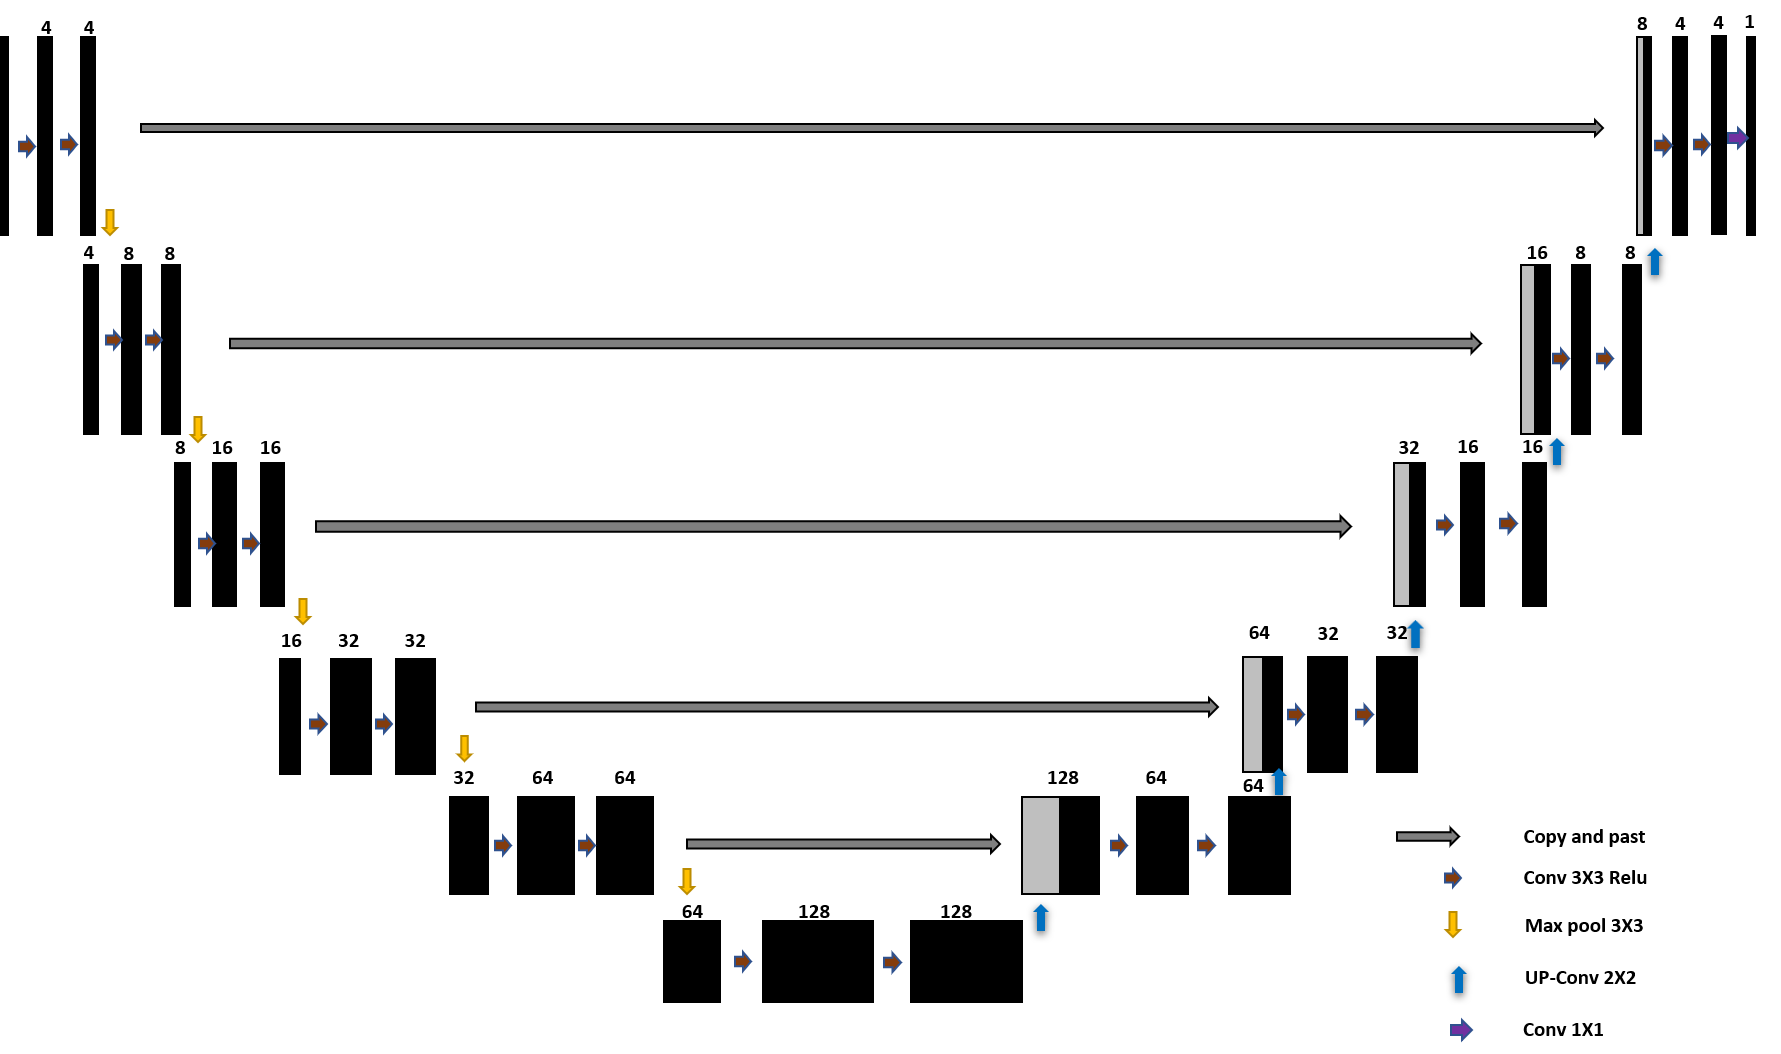
\includegraphics[scale = .3]{Picture1.png}
\caption{U-Net Lite a scale down version of U-net architecture}
\label{fig .2}
\end{figure}

While U-Net Lite sacrifices some modeling capacity compared to the original U-Net, it still provides a practical solution for various segmentation tasks in resource-constrained environments. Its reduced complexity makes it suitable for real-time applications and deployment on devices with limited computational capabilities.\\


\section{Quantum Powered U-Net}
The Quantum powered U-Net is an enhanced version of the U-Net architecture that incorporates quantum computing principles to improve its capabilities. In this variant, the bottleneck block of the U-Net, which is responsible for feature compression and expansion, is replaced with a quantum variational circuit. This quantum circuit introduces quantum operations and parameters that are trainable during the model optimization process.\\

The key technique used in the Quantum powered U-Net is the Amplitude embedding. Amplitude embedding is a method that encodes classical data into the amplitudes of quantum states. In the context of the Quantum powered U-Net, the information from the bottleneck block is encoded using the Amplitude embedding technique, allowing it to be processed by the quantum variational circuit.\\

To make the implementation more practical with current noisy quantum devices, the Quantum powered U-Net utilizes only seven qubits and a circuit depth of 9. This reduction in qubit count and circuit depth helps to mitigate the impact of noise and errors inherent in current quantum hardware.\\

During training, the parameters of the quantum variational circuit are optimized using quantum optimization algorithms or classical optimization techniques. This optimization process aims to find the best configuration of the quantum circuit that minimizes a predefined loss function, which is typically related to the quality of the segmentation results.\\

By integrating quantum computing into the U-Net architecture, the Quantum powered U-Net aims to leverage the unique computational properties of quantum systems, such as superposition and entanglement, to enhance the segmentation capabilities. The quantum variational circuit introduces additional expressivity and flexibility to capture complex relationships and patterns in the data, potentially leading to improved segmentation accuracy.\\

\begin{figure}[]

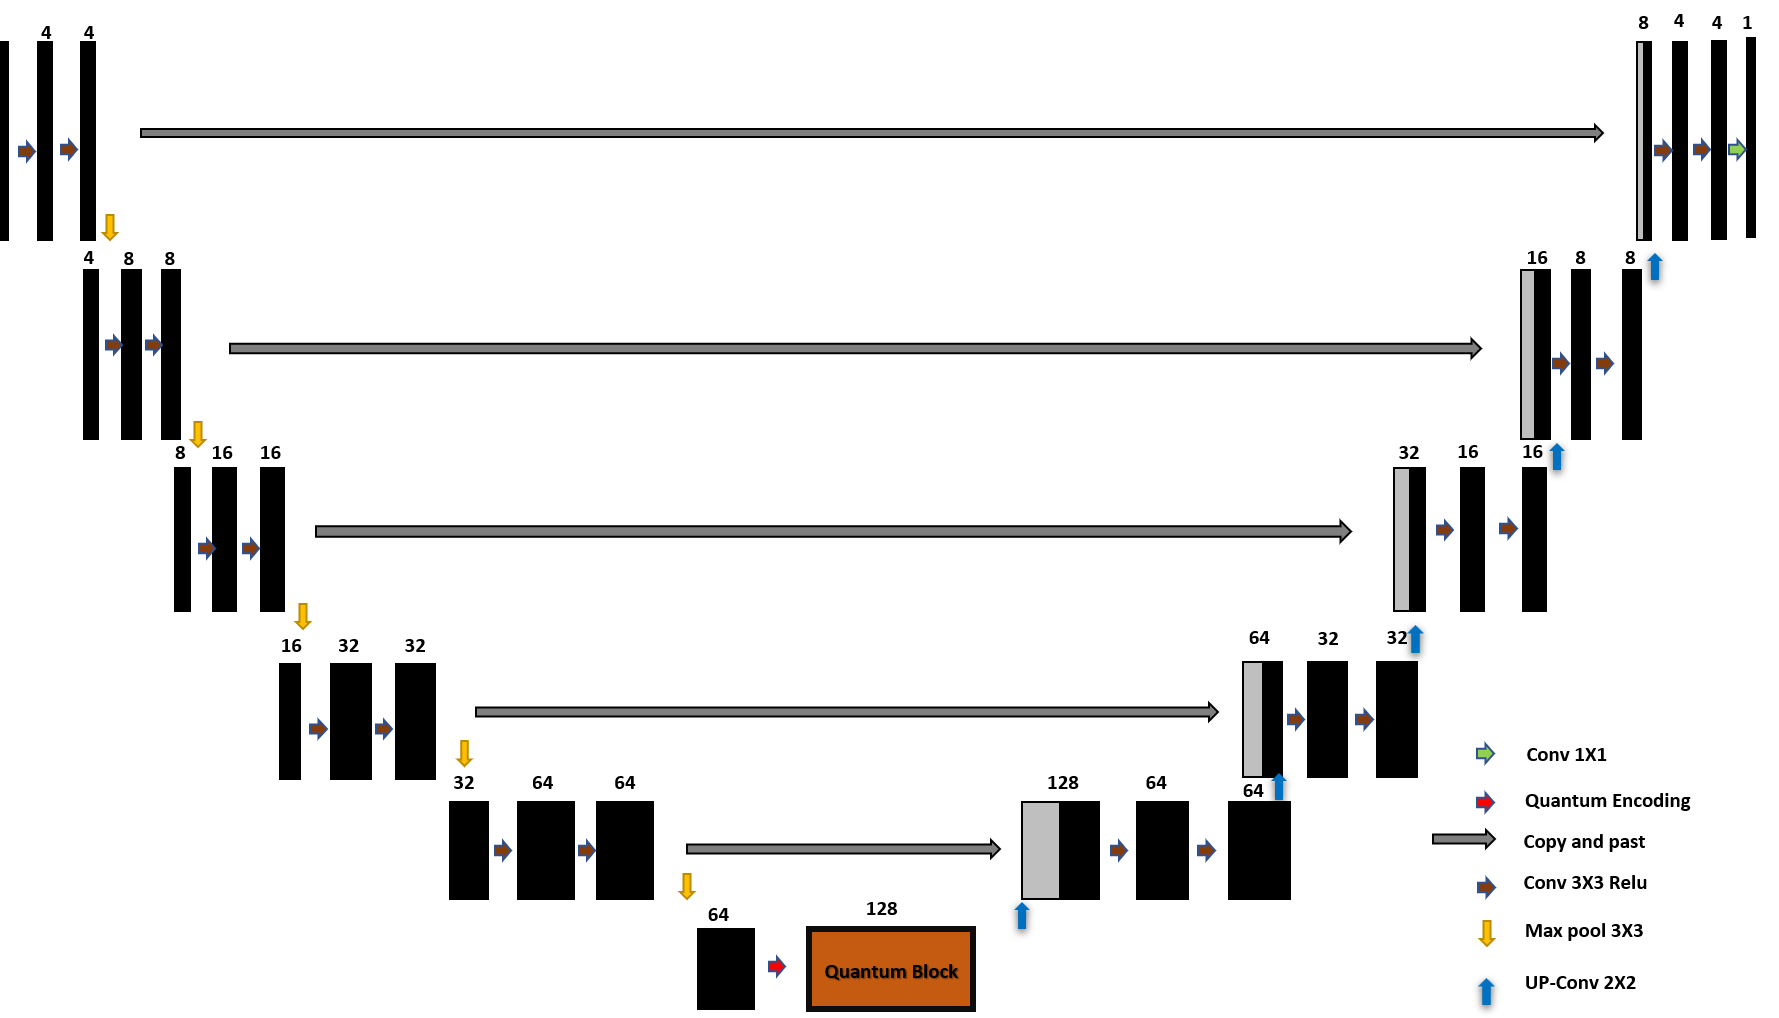
\includegraphics[scale = .3]{Picture2.png}
\caption{U-Net Lite a scale down version of U-net architecture}
\label{fig .2}
\end{figure}

It's important to note that the implementation of the Quantum powered U-Net is still subject to the limitations and challenges of current quantum hardware, including noise, limited qubit count, and imperfect gate operations. However, by using a reduced number of qubits and a shallower circuit, the Quantum powered U-Net aims to strike a balance between practicality and leveraging quantum computing advantages.\\














\section*{Acknowledgements\label{qnn_acknowledgements}}


\bibliographystyle{unsrt}
%\bibliographystyle{plain}
\bibliography{Reference/Ref}
\end{document}
